\documentclass[oneside]{book}
\usepackage{tests-tex-notebook}

\begin{document}

\chapter{Case with numbers}

\begin{mdcell}
We start from *the most simple* case possible, the case of numbers.

Note that this content is typed in markdown, and then converted to LaTeX via the `markdown` package.
\end{mdcell}

\begin{pycell}
x = 1
y = 2
\end{pycell}

\begin{pycell}
z = 3; n = 4
\end{pycell}

\begin{pycell}
l = 6
m = 7
\end{pycell}

\begin{mdcell}
We can print a linear combination of the provided number from a pycell, either directly...
\end{mdcell}

\begin{pycell}
print(x + y + z + n - l - m)
\end{pycell}
\begin{pyexpectedoutput}
-3
\end{pyexpectedoutput}

\begin{mdcell}
... implicitly ...
\end{mdcell}

\begin{pycell}
x + y + z + n - l - m
\end{pycell}
\begin{pyexpectedoutput}
-3
\end{pyexpectedoutput}

\begin{mdcell}
... or in both ways (with duplicated output)
\end{mdcell}

\begin{pycell}
print(x + y + z + n - l - m + 1)
x + y + z + n - l - m + 2
\end{pycell}
\begin{pyexpectedoutput}
-2
-1
\end{pyexpectedoutput}

\begin{mdcell}
One can also print lists of numbers
\end{mdcell}

\begin{pycell}
x = [1, 2, 3]
y = [4, 5, 6]
print(f"{x}")
print(f"{y}")
\end{pycell}
\begin{pyexpectedoutput}
[1, 2, 3]
[4, 5, 6]
\end{pyexpectedoutput}

\chapter{Case with strings and spaces}

\begin{mdcell}
One can print simple strings, possibly containing spaces
\end{mdcell}

\begin{pycell}
x = "one"
y = "two two"
\end{pycell}

\begin{pycell}
z = "three THREE_Three"; n = "FoUr_four quattro_cuatro"
\end{pycell}

\begin{pycell}
" ".join([x, y, z, n])
\end{pycell}
\begin{pyexpectedoutput}
'one two two three THREE_Three FoUr_four quattro_cuatro'
\end{pyexpectedoutput}

\begin{pycell}
print(" ".join([x, y]))
print(" ".join([z, n]))
\end{pycell}
\begin{pyexpectedoutput}
one two two
three THREE_Three FoUr_four quattro_cuatro
\end{pyexpectedoutput}

\begin{mdcell}
One can also print multiline strings
\end{mdcell}

\begin{pycell}
Z = """three
THREE_Three"""
N = """FoUr_four
quattro_cuatro"""
print("\n".join([Z, N]))
\end{pycell}
\begin{pyexpectedoutput}
three
THREE_Three
FoUr_four
quattro_cuatro
\end{pyexpectedoutput}

\begin{pycell}
Z = '''three
THREE_Three'''
N = '''FoUr_four
quattro_cuatro'''
print("\n".join([Z, N]))
\end{pycell}
\begin{pyexpectedoutput}
three
THREE_Three
FoUr_four
quattro_cuatro
\end{pyexpectedoutput}

\chapter{Variable resets}

\begin{mdcell}
In this file the python session resets at every chapter, and therefore
\end{mdcell}

\begin{pycell}
a = 1
b = "this is a string"
print(a, b)
\end{pycell}
\begin{pyexpectedoutput}
1 this is a string
\end{pyexpectedoutput}

\begin{mdcell}
works, but trying to use the variable `x` from the previous chapter would not (see `test_pycell_FAIL.tex`).
\end{mdcell}

\chapter{Figures}

\begin{mdcell}
You can have plotly figures in the code cells. By outputting the figure in the last line of the code cell it will be automatically added to the document.
\end{mdcell}

\begin{pycell}
import plotly.express as px
fig = px.scatter(x=[1, 2, 3], y=[4, 5, 6])
fig
\end{pycell}
\pyexpectedfigure{images/scatter_123_456.png}

\begin{mdcell}
A figure appears also when other text outputs are present
\end{mdcell}

\begin{pycell}
x = [10, 20, 30]
y = [40, 50, 60]
print(f"x = {x}")
print(f"y = {y}")
fig = px.scatter(x=x, y=y)
fig
\end{pycell}
\begin{pyexpectedoutput}
x = [10, 20, 30]
y = [40, 50, 60]
\end{pyexpectedoutput}
\pyexpectedfigure{images/scatter_102030_405060.png}

\chapter{Interacting with the outer document}

\texttt{mdcell} can interact with the rest of the document.

For instance, we can define an equation and a figure before the \texttt{mdcell} call.

\begin{equation}
1 + 1 = 2
\label{eq:1p1e2}
\end{equation}

\begin{figure}
\centering
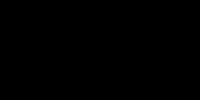
\includegraphics[width=0.5\linewidth]{images/fail_image_verification.png}
\caption{This is a sample figure with caption}
\label{fig:black}
\end{figure}

Next, we can refer to them inside the \texttt{mdcell} using \verb|`\eqref{...}`{=tex}| and \verb|`\ref{...}`{=tex}| commands.

\begin{mdcell}
We are inside the markdown cell: refer to `\eqref{eq:1p1e2}`{=tex} and to Figure `\ref{fig:black}`{=tex}.
\end{mdcell}

\chapter{Hiding codes}

When \texttt{PythonTeX} is loaded, by providing the optional \texttt{print} argument, some \texttt{pycell} can be executed, included in the output notebook, but hidden from the print.

We first show a cell without the \texttt{print} argument, which defines the variable \texttt{a} ...

\begin{pycell}
a = 1
\end{pycell}

... then a cell with \texttt{print=true}, which defines the variable \texttt{b} ...

\ifPythonTeXLoaded
\begin{pycell}[print=true]
b = 2
\end{pycell}
\else
\begin{pycell}
b = 2
\end{pycell}
\fi

... and finally a cell with \texttt{print=false}, which defines the variable \texttt{c} but will not show up in the pdf.

\ifPythonTeXLoaded
\begin{pycell}[print=false]
c = 3
\end{pycell}
\else
\fi

The variable \texttt{c} is still available, as we can see by summing \texttt{a + b + c}:
\begin{pycell}
a + b + c
\end{pycell}
\begin{pyexpectedoutput}
6
\end{pyexpectedoutput}

Unfortunately the \texttt{print} optional argument is not supported without \texttt{PythonTeX}.

\end{document}
